\documentclass[10pt]{article}

\usepackage[T1]{fontenc}
\usepackage{geometry}
\usepackage{amsmath, amssymb, amsthm}
\usepackage{array} 
\usepackage{enumitem}
\usepackage{siunitx}
\usepackage{graphicx}
\usepackage{caption}

\geometry{a4paper, margin=1in}
\setlength\parindent{0pt}
% \renewcommand\qedsymbol{$\blacksquare$}
\newcolumntype{L}{l@{\quad\quad}}
\newcounter{prob}
\def\problem{\stepcounter{prob}\paragraph{Problem \arabic{prob}}}
\def\solution{\\\\\textbf{Solution }}

\begin{document}
        \par\textbf{IISER Kolkata} \hfill \textbf{Assignment II}
        \vspace{3pt}
        \hrule
        \vspace{3pt}
        \begin{center}
                \LARGE{\textbf{ES1201 : Earth System Processes}}
        \end{center}
        \vspace{3pt}
        \hrule
        \vspace{3pt}
        Satvik Saha, \texttt{19MS154}\hfill\today
        \vspace{20pt}

        \problem Explain why heating an air parcel causes it to rise.
        \solution Heating an air parcel causes its density to decrease. This can be explained by the fact that supplying heat to air molecules
        increases their average kinetic energy, making the air parcel expand in volume. This less dense air is more buoyant than the surrounding
        cooler air, and hence rises upwards. Conversely, when an air parcel is cooled, it sinks.

        \problem Explain why the distribution of solar energy varies with latitude.
        \solution The incoming solar energy varies with latitude because of the curvature of the Earth's surface facing the Sun.
        The region where the incoming solar radiation strikes perpendicularly receives the maximum amount of solar energy (this is close to the equator,
        but the latitude varies with the seasons due to Earth's axial tilt).
        Moving away from these regions, the Earth's surface slopes away, and thus each square metre of surface receives less solar energy
        (we could also say that the same amount of solar energy is distributed over larger areas).
        Hence, the higher latitudes receive in average a lower amount of solar energy.

        \begin{figure}[h!]
        \begin{center}
                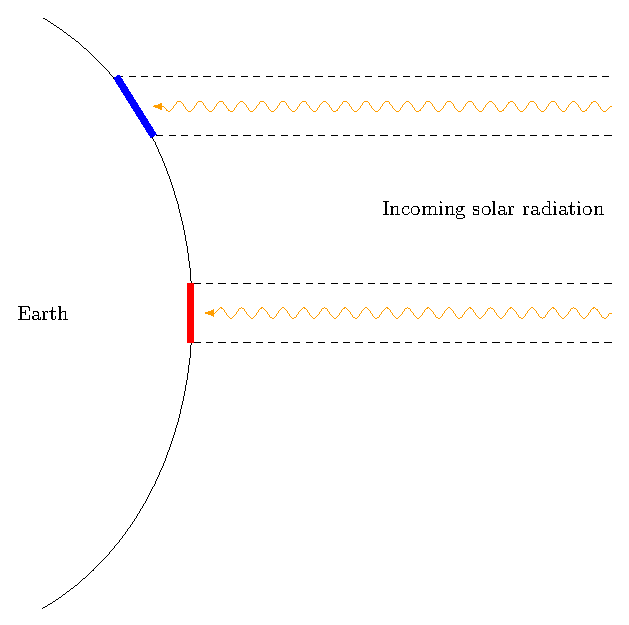
\includegraphics[scale=0.7]{./insolation.eps}
        \end{center}
        \caption*{\it The area over which the same amount of solar energy is distributed is clearly higher in the higher latitudes (blue),
        compared to the equatorial regions (red).}
        \label{fig:insolation}
        \end{figure}

        \problem Using a diagram, describe Hadley cells. Are they affected by seasonal variations? Explain briefly.
        \solution Hadley cells describe a pattern of large scale air circulation around the equator.
        A Hadley cell is essentially a convective cell, caused by the circulation of heating and cooling of air. The tropics experience
        a large amount of solar heating, so the surface heats up the overlying layer of air. This causes the sir to rise up, forming a zone
        of low pressure on the surface. This air is thus replaced by air moving towards the equator from regions of higher pressure.
        Now, the rising air can only move upwards as long as its temperature is more than that of surrounding air. Since air temperature
        rises with altitude in the troposphere, the rising air is forced to stop at a certain point and diverge away from the equator,
        towards the poles. This air eventually sinks at around \SI{30}{\degree} away on either side of the equator, replacing the air moving
        towards the equator. This entire cycle comprises a Hadley cell.\\

        Hadley cells form on either side of the intertropical convergence zone (ITCZ), which is the belt of converging air from the \SI{30}{\degree}
        latitudes and the rise of heated air from the tropics. During the summer in a particular hemisphere, the air temperature on
        that side of the equator will be higher than usual, due to the higher solar energy input in that hemisphere. Thus, the temperature gradient
        between the poles and the tropics decreases in that hemisphere. This in turn reduces the strength of atmospheric circulation on that side,
        hence the air circulation patterns move polewards where the temperature gradient is greater. This means that the Hadley cells and the ITCZ
        move towards the hemisphere experiencing summer, albeit with a small time lag.
        
        \begin{figure}[h!]
        \begin{center}
                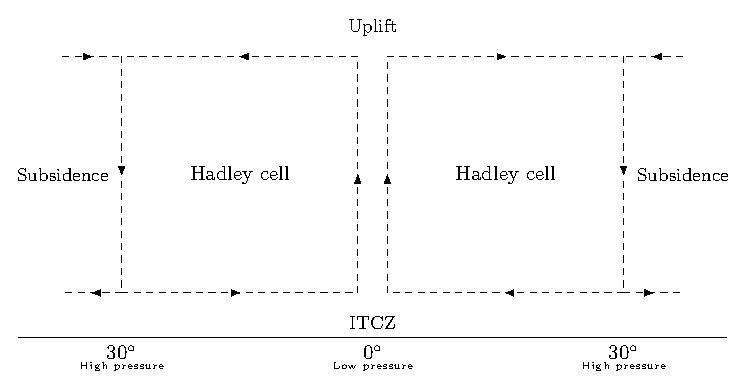
\includegraphics{./hadley.eps}
        \end{center}
        \caption*{\it Hadley cells adjoining the ITCZ.}
        \label{fig:hadley_cells}
        \end{figure}

        \problem What are the polar front zones? Explain their formation.
        \solution The polar front zones are zones of steep temperature gradients at around \SI{60}{\degree} N and S.
        They are formed by the collision of two masses of cold and warm air. The cold air is generated from the poles,
        where very low temperatures causes high density air to form near the surface. The high pressure leads cold air
        to diverge at the surface towards the equator. At the same time, this cold air subsides.
        The warm air is generated from the subtropics. These two air masses do not mix well, so the cold air sinks below the warm air,
        causing the polar front to slope upwards towards the poles.


        \begin{figure}[h!]
        \begin{center}
                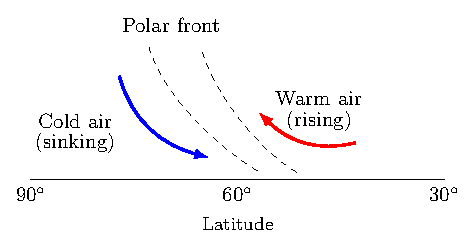
\includegraphics{./polar_front.eps}
        \end{center}
        \caption*{\it The formation of the polar front zones.}
        \label{fig:polar_front}
        \end{figure}
        

        \problem Explain why Earth experiences different seasons throughout the year.
        Which parts of Earth experience extreme variability and which parts experience the least? Explain why.
        \solution Earth's seasonal variation of temperature is primarily caused by its axial tilt, or obliquity of \SI{23.5}{\degree} from the
        perpendicular. Because of this, each hemisphere is tilted towards the Sun more than the other for a six month period, during which
        that hemisphere receives more solar energy on average. For example, the latitude which receives the maximum solar energy is the one
        where the Sun is directly overhead -- this varies between the Tropic of Cancer (\SI{23.5}{\degree}N) and the Tropic of
        Capricorn (\SI{23.5}{\degree}S). Thus, we see that in a narrow range of latitudes surrounding the equator, the Sun is always close to being
        directly overhead. These tropics thus receive a large amount of solar energy throughout the year, and hence have little seasonal
        variation in temperature. On the other hand, the poles receive six months of continuous sunlight in the summer, then six months of darkness in
        winter. Hence, the higher latitudes experience extreme variability in temperature with the change in season.\\

        Earth's seasonal variation is affected to a lesser degree by its changing distance from the Sun. Its elliptical orbit means that
        there is a closest point (perihelion) and a farthest point (aphelion).\\

        The seasonal variability is also much greater over land surfaces than over oceans, because of their different thermal properties.
        This phenomenon is called continentality. Simply put, land surfaces heat up and cool down faster than water (which has a large
        specific heat capacity, and waterbodies experience mixing between layers). Thus, the interiors of continents experience
        a greater seasonal temperature variation than coastal regions.

        \problem What is the intertropical convergence zone (ITCZ)? Explain why it moves northward and southward with seasonal shifts.
        \solution The ITCZ is a region of convergence and upward movement of air in the tropics. A large amount of solar energy is
        received in the tropics, which heats up the surface, in turn heating up the overlying air. This air rises upwards, thus forming a 
        belt of low pressure. To replace it, air moves along the surface from regions of higher pressure from both sides. This meeting
        of air masses is called convergence, and this zone of convergence in the tropics is the ITCZ. In addition, the heated air carries
        water vapour, which condenses as the air cools as it rises. This forms heavy cloud cover and precipitation.\\

        During seasonal shifts, the hemisphere which experiences summer receives more solar energy on average, and the region receiving
        maximum incoming solar energy shifts away from the equator towards the corresponding pole. Hence, the temperature gradient between
        the tropics and that pole decreases. This reduces the strength of atmospheric circulation, and circulation patterns shift polewards.
        In the winter, the reverse happens, as the other hemisphere now experiences summer. The ITCZ thus moves polewards towards the 
        hemisphere experiencing summer, with a time lag. This means that the low pressure belt, corresponding to the belt of maximum heating,
        moves with the seasons.

        \problem How are jet streams formed? Briefly explain the physics of their formation.
        \solution Jet streams are high speed winds in the upper troposphere in the midlatitudes. They are a result of the pressure gradient
        in the troposphere between different latitudes. The air in the tropics is relatively warmer in the tropics than at the poles,
        so the troposphere is thicker at the tropics than at the higher latitudes. Thus, at a given altitude, the pressure decreases
        as we move towards the poles. This pressure gradient is the steepest at the midlatitudes, hence the wind speed is greatest.
        Now, the Coriolis force causes a horizontal movement towards the east, so these winds have a westerly component.
        The pressure gradient force and the Coriolis force, which are opposing, result in a net movement of air perpendicular
        to the pressure gradient, called geostrophic wind. This flow is also affected by factors such as centripetal and centrifugal
        forces from curved paths, the presence of high and low pressure zones and friction from the Earth's surface. ({\it The latter is 
        largely irrelevant in the upper troposphere, so the flow there is mostly geostrophic.})

        \problem Explain continentality.
        \solution Oceans absorb much more solar energy than land, because of its lower albedo. In addition, heat absorbed by oceans
        is rapidly transferred downwards due to mixing, and upwards into the atmosphere by convection. Land also loses heat to 
        the atmosphere, but transfers heat downward by conduction much more slowly. Furthermore, the specific heat capacity
        of water is much higher than of dry soil, i.e.\ water can absorb much more heat than soil for the same rise in temperature.
        Hence, land surfaces heat up much more quickly, and cool down much more rapidly than oceans. This has effects on daily
        (land and sea breezes) as well as seasonal timescales. The greater thermal variability of land means that the interior of
        continents experience greater seasonal temperature extremes than coastal regions, where the oceans provide a moderating effect.
        This phenomenon is called continentality.

        \problem Explain why the greatest thermal variations are found in the interior of large continental masses,
        and the lowest variations over the tropical oceans.
        \solution This is because of two factors -- the lower seasonal variability of tropical regions than in higher latitudes,
        and the moderating effect of oceans, i.e.\ continentality. Tropical oceans act as reservoirs of heat due to the high specific heat
        of water and mixing between the layers of water. Hence, they release heat during winters and absorb heat during summers,
        reducing temperature extremes in comparison to the interiors of continents. In addition, the tropics receive roughly the same
        amount of solar energy throughout the year, as the Sun is almost always vertically overhead. Hence, tropical oceans
        experience much more moderate seasonal variations.

        \problem Describe three processes that produce uplift in the atmosphere and are important in causing precipitation.
        \solution Three processes which produce uplift in the atmosphere are as follows.
        \begin{enumerate}[label=(\roman*), itemsep=0pt, topsep=\parsep]
                \item \textit{Convection:} Typically, land surfaces heated by incoming solar radiation heats the layer of air just above it.
                Heated air becomes less dense than colder air, and thus rises. Colder air sinks and moves in to replace it.
                This in turn heats up, thus completing the cycle. If the rising air carries water vapour (evaporated from some waterbody),
                this condenses when the air reaches a certain height and cools down. This leads to cloud formation, and eventually precipitation.
                An example of this process is heavy precipitation in the ITCZ, where uplift is caused by convection cells (Hadley cells).

                \item \textit{Mixing of air masses.} Air masses of different densities (typically different temperatures too) moving towards each
                other do not mix well. Instead, the lighter air mass moves over the denser air mass, thus forming a sloping interface or front.
                Thus, the lighter/warmer air is forced upwards. Again, if this air carries water vapour, this leads to cloud formation and precipitation.
                An example of this is the formation of the polar front zones, where the temperatures of the meeting air masses are very different
                as one arrives from the poles and the other from the tropics.

                \item \textit{Topography.} Land features, primarily mountain ranges, can force the upward movement of air. When moisture carrying
                air (perhaps obtained from evaporation over a waterbody) strikes the face of a mountain range, it moves upwards and 
                cools down. This causes condensation of the moisture, and hence heavy precipitation on the windward slope of the mountains.
                This phenomenon is called orographic precipitation. An example of this is the heavy rainfall experienced in the Western Ghats
                of India.
        \end{enumerate}

\end{document}
